\noindent
This project focuses on the Mars Sample-Return Rover, developed by NASA's Jet Propulsion Laboratory (JPL). Exploring the unknown is fascinating with the challenges that are present. Robotics is a field suitable to approach these challenges because they have the capability to operate autonomously. The model will be created in Solidworks and then simulated in Gazebo. The report explains the elements of the project, starting with the rover's geometric aspects such as its mechanical design, joints, links, and arm. The rover consists of the vehicle base with the chassis and wheels, and an attached four degree-of-freedom (4DOF) arm.\\

The rover's chassis has an interesting structure with the front and rear links are connected with one joint, but have independent movement. With a total range of 180 degrees, the rover can scale steep cliffs because of the design. The front wheels can also rotate side-to-side so that the rover can turn. Attached to the chassis is a 4DOF arm. It rotates at its base, an elbow joint, and the wrist joint can rotate sideways and and up and down. The end-effector on the arm allows for sample-collection. \\

With the challenges of unknown terrain and inability to remote control the robot, extensive research and testing has to be made before launching the robot. The scope of this project focuses on the Sample-Return Rover. Model assumptions will be discussed. Afterwards, the design of the robot will be explained with analysis of the kinematics of the vehicle and the arm.

\begin{figure}[htb]
	\centering
	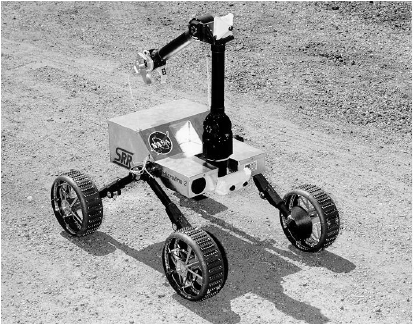
\includegraphics[scale=0.70]{sections/introduction/images/srr.png}
	\label{sample_return_rover:introduction:sample_return_rover}
	\caption{Early Model of the Sample Return Rover}
\end{figure}


\chapter{Motivation}
Space robotics is a big area of interest. Not only has there been the Sample-Return Rover, but there is also the CubeSat, BioSentinel, and many others. The Sample-Return Rover is a great choice for this project as the information gained from the class will be used on the rover. There are many possible usages for space robotics. They can serve the purpose of exploring unknown territory, surveillance of the Earth, or maintenance on existing robots/satellites.  \\

Each different type of robot will deal with their own challenges, whether it is dealing with low or zero gravity, extreme temperature changes, or rocky terrain. It is amazing how diverse space robotics can be. The area of research is vast and takes much effort to be in a robotics field. The intention of this project is to get an introductory hands-on experience with both mobile robots and a manipulator simulation. Calculating forward, inverse, and velocity kinematics are a big topic for this project, as well as implementation of those calculations into algorithms. 



\chapter{Assumptions}
Since the scope of this project deals with simulating a robot in outer space, there are assumptions to be made because certain things cannot be measured easily. To deal with this issue and other design factors, there are assumptions to follow. 

\begin{enumerate}
	\item The robot is a rigid body, any torque or force acted upon any link will not be deformed.
	\item The steering design is based off the Ackermann-Steering model.
	\item All motion or revolution will be around the z-axis.
	\item The simulations will be in Gazebo and RVIZ. 
\end{enumerate}